\documentclass[a4paper]{article}
\usepackage[utf8]{inputenc}
\usepackage[T1]{fontenc}
\usepackage{lmodern}
\usepackage{listings}
\usepackage{graphicx}
\usepackage{dirtree}
\usepackage{caption}
\usepackage{subcaption}
\usepackage{float}
\usepackage[english]{babel}
\usepackage[margin=1.1in]{geometry}
\title{Localizer User Manual}
\author{\textsc{SIPP Florian}}
\lstset{
	frame = single,
	basicstyle = \footnotesize\ttfamily
}

\begin{document}
\maketitle
\begin{abstract}
This document is the user manual of the Software Localizer. Localizer is being developed by the Centre de Recherche en Neurosciences de Lyon (CRNL) to allow the quick analysis of data recovered during Localizer tasks performed by iEEG patients before their possible surgery due to drug resistant epilepsy.  Localizer is also the term used to define a set of tasks requiring the use of specific cognitive abilities. Those tasks will allow the researcher or the clinician to check for indications of epileptic activity in specific areas of the brain. 
\end{abstract}
\tableofcontents
\newpage
\section{Data Curation} \label{curation}    
\paragraph{} In order to get the most of Localizer you can organize your data in several ways which are going to be described.
\subsection{Subject Folder organisation}
\begin{figure}[H]
\framebox[\textwidth]{%
\begin{minipage}{0.9\textwidth}
\dirtree{%
	.1 HOSPITAL{\_}YEAR{\_}PATID/.
	.2 HOSPITAL{\_}YEAR{\_}PATID{\_}TASK1/.
	.3 HOSPITAL{\_}YEAR{\_}PATID{\_}TASK1.TRC.
	.3 ....
	.2 HOSPITAL{\_}YEAR{\_}PATID{\_}TASK2/.
	.3 HOSPITAL{\_}YEAR{\_}PATID{\_}TASK2.TRC.
	.3 ....
	.2 HOSPITAL{\_}YEAR{\_}PATID{\_}TASK3/.
	.3 HOSPITAL{\_}YEAR{\_}PATID{\_}TASK3.TRC.
}
\end{minipage}
}
\caption{\label{SubjectDirectory}Subject directory hierarchy}
\end{figure}
\subsection{Multiple Subjects Folder}
\begin{figure}[H]
\framebox[\textwidth]{%
\begin{minipage}{0.9\textwidth}
\dirtree{%
	.1 YEAR1.
	.2 HOSPITAL{\_}YEAR1{\_}PATID/.
	.3 HOSPITAL{\_}YEAR1{\_}PATID{\_}TASK1/.
	.4 HOSPITAL{\_}YEAR1{\_}PATID{\_}TASK1.TRC.
	.4 ....
	.3 HOSPITAL{\_}YEAR1{\_}PATID{\_}TASK2/.
	.4 HOSPITAL{\_}YEAR1{\_}PATID{\_}TASK2.TRC.
	.4 ....
	.3 HOSPITAL{\_}YEAR1{\_}PATID{\_}TASK3/.
	.4 HOSPITAL{\_}YEAR1{\_}PATID{\_}TASK3.TRC.
	.1 YEAR2.
	.2 HOSPITAL{\_}YEAR2{\_}PATID/.
	.3 HOSPITAL{\_}YEAR2{\_}PATID{\_}TASK1/.
	.4 HOSPITAL{\_}YEAR2{\_}PATID{\_}TASK1.TRC.
	.4 ....
	.3 HOSPITAL{\_}YEAR2{\_}PATID{\_}TASK2/.
	.4 HOSPITAL{\_}YEAR2{\_}PATID{\_}TASK2.TRC.
	.4 ....
	.3 HOSPITAL{\_}YEAR2{\_}PATID{\_}TASK3/.
	.4 HOSPITAL{\_}YEAR2{\_}PATID{\_}TASK3.TRC.
}
\end{minipage}
}
\caption{\label{MultipleSubjectsDirectory}Multiple Subjects directory hierarchy}
\end{figure}
\subsection{EEG Files Folder}
\begin{figure}[H]
\framebox[\textwidth]{%
\begin{minipage}{0.9\textwidth}
\dirtree{%
	.1 ROOT{\_}FOLDER.
	.2 my{\_}awesome{\_}file.TRC.
	.2 file{\_}frOm{\_}Collab.eeg.
	.2 file{\_}frOm{\_}Collab.vhdr.
	.2 file{\_}frOm{\_}Collab.vmkr.
	.2 another{\_}file.edf.
}
\end{minipage}
}
\caption{\label{MiscEEGDirectory}Folder with eeg files without structure}
\end{figure}
\subsection{BIDS Subject Folder}
\begin{figure}[H]
\framebox[\textwidth]{%
\begin{minipage}{0.9\textwidth}
\dirtree{%
	.1 BidsDataset.
	.2 code.
	.2 dataset{\_}description.json.
	.2 derivatives.
	.2 participants.tsv.
	.2 sub-6d5ecf1a54f9.
	.3 ses-post.
	.4 anat.
	.4 ieeg.
	.5 sub-6d5ecf1a54f9{\_}ses-post{\_}task-VISU{\_}channels.tsv.
	.5 sub-6d5ecf1a54f9{\_}ses-post{\_}task-VISU{\_}events.tsv.
	.5 sub-6d5ecf1a54f9{\_}ses-post{\_}task-VISU{\_}ieeg.eeg.
	.5 sub-6d5ecf1a54f9{\_}ses-post{\_}task-VISU{\_}ieeg.json.
	.5 sub-6d5ecf1a54f9{\_}ses-post{\_}task-VISU{\_}ieeg.vhdr.
	.5 sub-6d5ecf1a54f9{\_}ses-post{\_}task-VISU{\_}ieeg.vmrk.
	.3 ses-pre.
	.4 anat.
	.4 ieeg.
	.2 sub-c5c66d0e5eca.
	.3 ses-post.
	.4 anat.
	.4 ieeg.
	.5 sub-c5c66d0e5eca{\_}ses-post{\_}task-MVIS{\_}channels.tsv.
	.5 sub-c5c66d0e5eca{\_}ses-post{\_}task-MVIS{\_}events.tsv.
	.5 sub-c5c66d0e5eca{\_}ses-post{\_}task-MVIS{\_}ieeg.eeg.
	.5 sub-c5c66d0e5eca{\_}ses-post{\_}task-MVIS{\_}ieeg.json.
	.5 sub-c5c66d0e5eca{\_}ses-post{\_}task-MVIS{\_}ieeg.vhdr.
	.5 sub-c5c66d0e5eca{\_}ses-post{\_}task-MVIS{\_}ieeg.vmrk.
	.3 ses-pre.
	.4 anat.
	.4 ieeg.
}
\end{minipage}
}
\caption{\label{BidsDirectory}Structure of folder containing BIDS formated data}
\end{figure}
\section{Options} \label{options}    
\subsection{Localizer}
\paragraph{} This option menu will let you create .prov files. The .prov extension stands for \textbf{protocol visualization}. Typically, a Localizer is a set of time series (one for each channel) with data for each sample from the beginning to the end of the recording session. In addition,  information about the events of the experimental paradigm is stored, each event being identified using a code (e.g. an event of code 10 occured at sample 134567).
\paragraph{} The .prov file instructs Localizer on how to epoch the data based on the events. It consists of blocs which contain a list of subblocs. Each bloc or subbloc will be sorted using first their respective order and then alphabetically using their respective names.
\paragraph{} Each subbloc is centered around a specific event, called \textbf{main event}, for a specific time window (for instance, consider all events with code 10 and extract for each of them a window ranging from 200ms before to 700ms after that event). You can specify secondary events which do not interfere in the epoching. You can also set a baseline window, which is used for statistical analysis.
\paragraph{} Each bloc also has a sorting method, which is used to sort the trials obtained from the epoching according to specific conditions (code of the main event, latency of the secondary event...). The syntax used here for a condition is \textit{SUBBLOC{\_}EVENT{\_}COMMAND} where SUBBLOC is the name of the sub-bloc, EVENT the name of the event and COMMAND the sorting parameter (which can be LATENCY or CODE). You can specify multiple conditions which are separated by a semi-colon, each of which are interpreted in the order they have been written. The rest of the .prov file is straightforward: you can specify images (.png or .jpg) at specific time windows, or to associate an image to a bloc. 
\subsection{File Priority}
\paragraph{} In The case of non BIDS datasets , you might have some of your data in a specific format , let's say Micromed TRC for instance and you receive some Brainvision data . The file priority options will allow you to say , i want you to search first for Micromed data , then for Brainvision data and will allow you to deal with multiple file formats without having to go through lengthy conversion steps.
\subsection{Statistic}
\paragraph{} For each type of data representation, there will be at the same time some statistical analysis processed during the creation of the maps:

\begin{itemize}
\item a paired difference test,  more commonly known as Wilcoxon.
\item a non paired difference test,  more commonly known as Kruskall-Wallis.
\end{itemize}

For each of those test you will be abble to choose the P value that you estimate will draw out the significant value of your data as well as a choice beetween analysing your data just with the P Value or using a false discovery rate (FDR) correction.

For Kruskall-Wallis statistic, you will also have the choice to use the parameter \textbf{Bloc wise statistics},  it will [BLABLABLA revoir les mails de JP ou revoir dans le code directement ce que ca fait]
\subsection{Pictures}
\paragraph{} These options will allow you to choose the width or the height of the generated pictures. In order to keep an optimal representation, a ratio is automatically applied when you choose a custom width or heigth.

For the trial matrices you can choose an interpolation factor in order to produce maps of better quality. The bigger the ratio the longer the time it will take to generate the maps, the default value is what we feel is the best ratio beetween generation time and picture quality.
\subsection{Frequency Bands}
\paragraph{} In order to process the Hilbert Envelope of a signal you will use this window to define your bands of interest. 
For each wanted frequency band, simply add a new element and define : 
\begin{itemize}
\item Label : Name of your frequency band, it will be used in the main user interface
\item Frequency minimum : The lower bound of your frequency range of interest
\item Frequency step : The step which will be used to divide the entire range during the analysis
\item Frequency maximum : The higher bound of your frequency range of interest
\end{itemize}

\paragraph{} Let's say i want to define a High Gamma frequency range going from 50 to 150Hz with steps of 10Hz,  i will simply input :
\begin{itemize}
\item Label : Gamma
\item Frequency minimum : 50
\item Frequency step : 10
\item Frequency maximum : 150
\end{itemize}
\section{Data Analysis} \label{analysis}    
\subsection{Hilbert Transform}
\paragraph{} The signal for each contact was first bandpass‐filtered in multiple successive 10 Hz wide frequency bands (e.g. 10 bands from [50–60 Hz] to [140–150 Hz]) using a zero phase shift no causal finite impulse filter with 0.5 Hz roll‐off. The envelope of each bandpass‐filtered signal was then computed with a standard Hilbert transform then down‐sampled to 64 Hz and divided by its means across the entire recording session and multiplied by 100, to express each value as a percentage of that mean (normalization).  

\begin{figure}[H]
\begin{center}
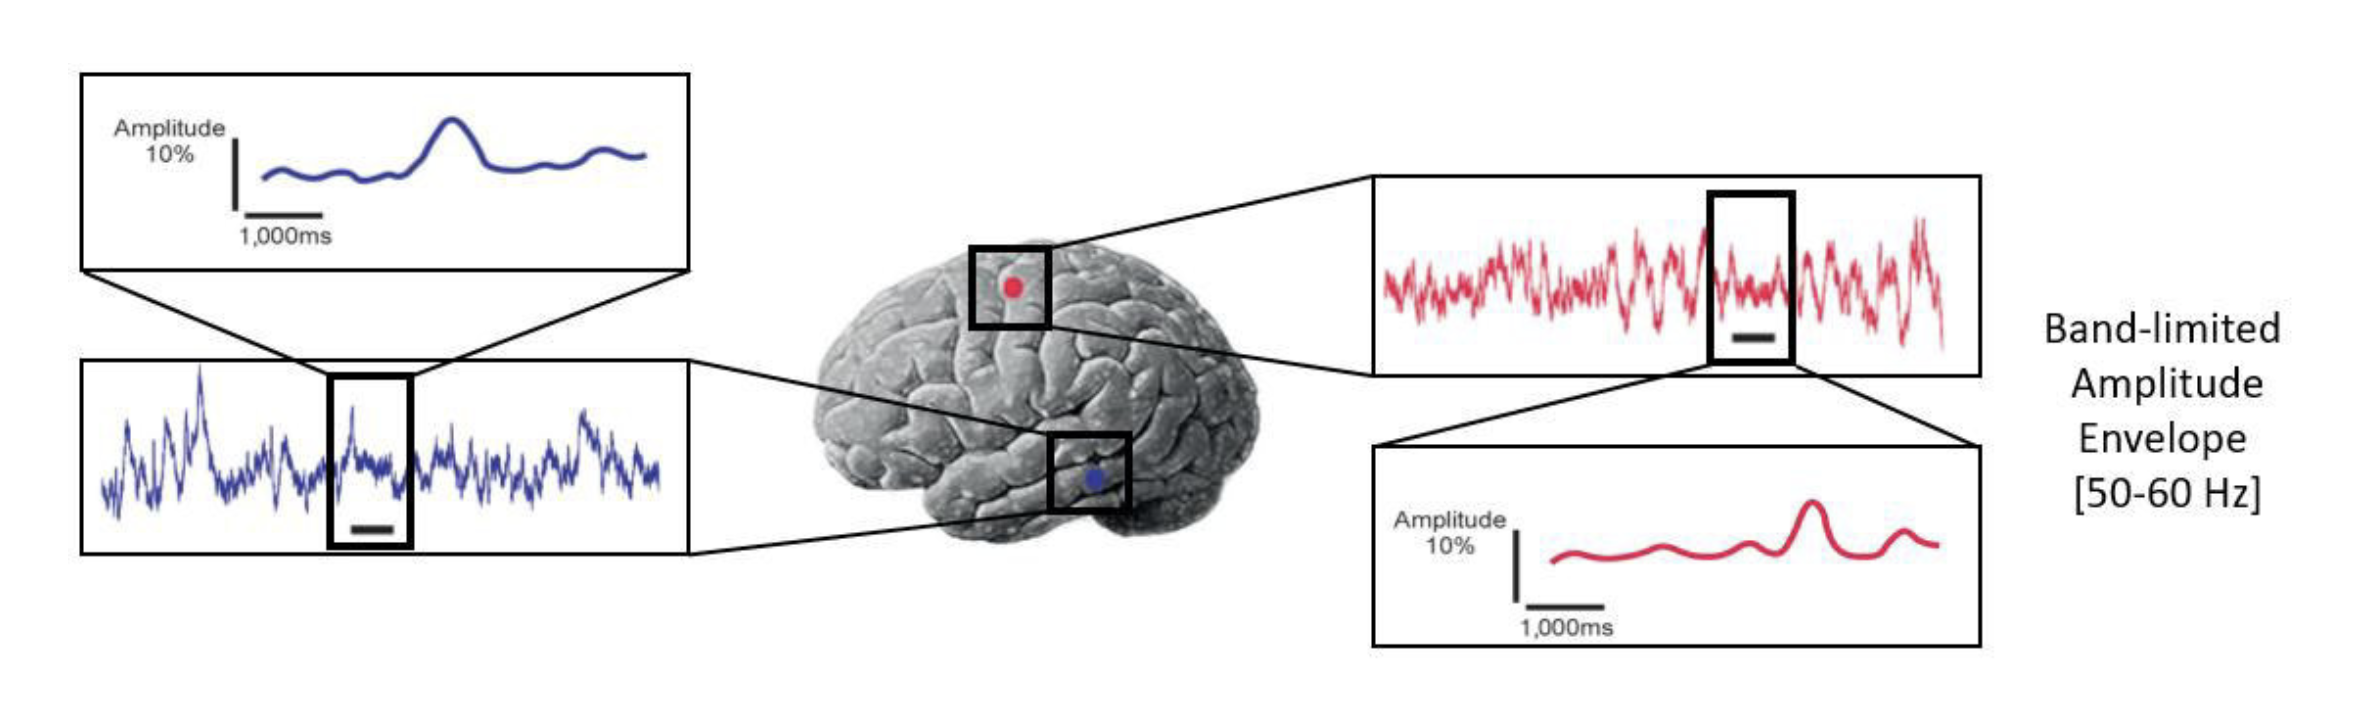
\includegraphics[scale=0.4]{HilbertProcessing.png}
\end{center}
\caption{\label{HilbertProcessingPicture}Hilbert Transform of raw IEEG Data}
\end{figure}

Finally, the normalized envelope signals for each of the ten frequency band were averaged together to provide a single HFA signal. By construction, the mean value of that HFA signal across the entire recording session is equal to 100. The whole procedure is also designed to reduce the 1/f drop‐off in amplitude of the raw iEEG signals. 

\subsection{Envelope Plot}
\paragraph{} Still blabla
\begin{figure}[H]
\begin{center}
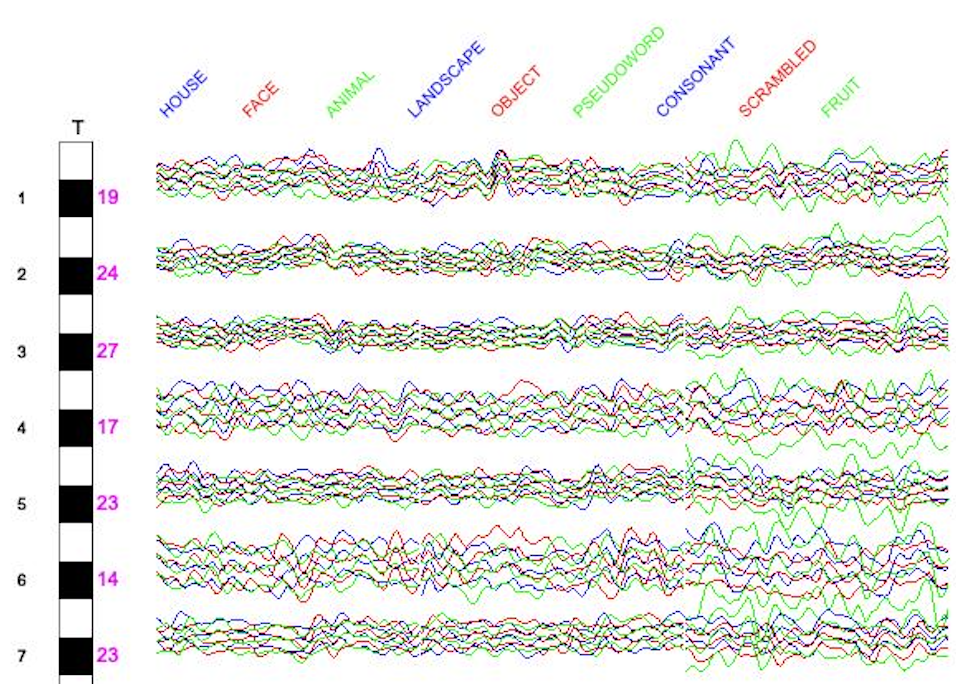
\includegraphics[scale=0.8]{EnvelopePlots.png}
\end{center}
\caption{\label{EnvelopePlotsPicture}Gamma Band activity for each contact and each conditions during the visual task}
\end{figure}
\subsection{Time Trials Matrices}
\paragraph{} Still blabla
\begin{figure}[H]
\begin{center}
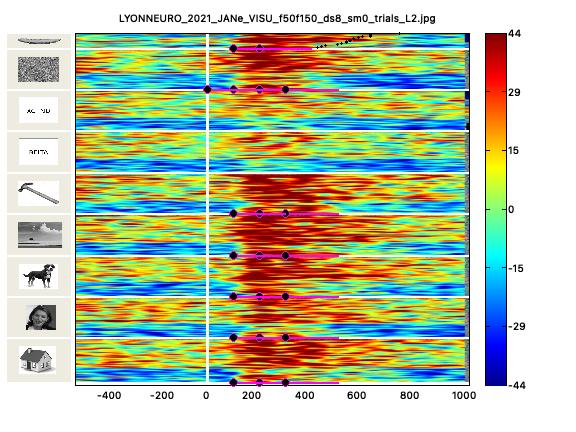
\includegraphics[scale=0.7]{TimeTrialsMatrice.jpg}
\end{center}
\caption{\label{TimeTrialsPicture}Gamma Band activity during the visual task}
\end{figure}
\subsection{Correlation Maps}
\paragraph{} Still blabla
\subsection{Statistical Files}
\paragraph{} Still blabla
\section{Tutorials} \label{tutorials}    
\subsection{Processing data from a subject folder}
\paragraph{} The si
\subsection{Processing data from a multiple subjects folder}
\subsection{Processing data from an EEG files folder}
\subsection{Processing data from a BIDS subject folder}

\end{document}